\documentclass[a4paper]{article}

\usepackage[pdftex]{graphicx}
\usepackage[margin=3cm]{geometry}
\usepackage{verbatim,moreverb,amssymb,amsmath}


\newcounter{question}
\newcommand{\question}[1]{\refstepcounter{question}\section*{Question~\thequestion~~~\small\emph{(#1)}}}
\renewcommand*\thequestion{\arabic{question}}


\begin{document}

\pagestyle{empty}
\thispagestyle{empty}



\noindent
\begin{minipage}{\columnwidth}
  \centering
  \Large
  DA4002 (HT11) Halmstad University\\
  Introduction to Algorithms, Data Structures, and Problem Solving\\[3\baselineskip]
  \Huge
  Written Exam\\
  \Large
  Thursday, January 10, 2013\\[2\baselineskip]
  Examiner: Roland Philippsen
\end{minipage}

\vfill

\noindent
\begin{center}
\fbox{
  \begin{minipage}{0.8\columnwidth}
    \textbf{Student Name:}\\[3\baselineskip]
  \end{minipage}
}
\end{center}

\vfill



\section*{Rules}

Aside from the obvious rules of conduct exams (e.g.\ no chatting):

\begin{itemize}
\item
  \textbf{No computing devices} (laptops, phones, calculators, \emph{etc}).
\item
  \textbf{No books or printouts} except for non-electronic dictionaries.
\item
  \textbf{Allowed hand-written notes}: two sheets of A4 paper (front and back).
\end{itemize}



\section*{General Guidelines}

\begin{itemize}
\item
  \textbf{Read carefully} and pace yourself.
  You can solve the problems in any order you want, but later problems may be easier to solve after you have answered the preceding questions.
\item
  \textbf{Write clearly} and draw clear diagrams.
  If you need to correct a mistake, then cleanly cross out the wrong answer and clearly indicate where the correction can be found.
\item
  \textbf{Indicate the question number} for each of your answers.
  If a question has sub-questions, indicate the sub-question number after the main question number, separated by a dot.
  For example, question 3 has 4 sub-questions, and their answers should be numbered 3.1, 3.2, 3.3, and 3.4.
\end{itemize}



\pagebreak
\pagestyle{plain}
\thispagestyle{plain}
\setcounter{page}{1}



\question{6 points}

Below are six diagrams labelled \textbf{(A)}, \textbf{(B)}, \textbf{(C)}, \textbf{(D)}, \textbf{(E)}, and \textbf{(F)}.
Each of them shows a data structure containing items of value $\{1, 2, 3, 4, 5, 6, 7\}$.

\vfill

\begin{center}
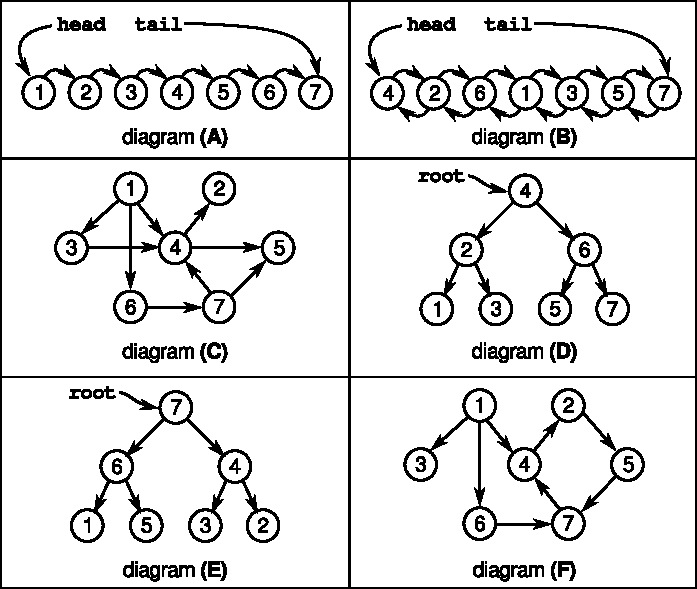
\includegraphics[width=0.8\columnwidth]{ds.pdf}
\end{center}

\vfill

\noindent
Match each data structure diagram with one of the data structure names in the table below.
Use the most specific data structure name for each diagram.

\vfill

\begin{center}
  \begin{tabular}{|p{0.3\columnwidth}|p{0.3\columnwidth}|}
    \hline
    data structure name & diagram label \\
    \hline
    & \\
    \textbf{singly linked list} & \\
    & \\
    \hline
    & \\
    \textbf{doubly linked list} & \\
    & \\
    \hline
    & \\
    \textbf{binary search tree} & \\
    & \\
    \hline
    & \\
    \textbf{max heap} & \\
    & \\
    \hline
    & \\
    \textbf{directed graph} & \\
    & \\
    \hline
    & \\
    \textbf{directed acyclic graph} & \\
    & \\
    \hline
  \end{tabular}
\end{center}


\clearpage


\question{10 points}

Answer the following questions about computational complexity.

\begin{enumerate}
  
\item
  Algorithm \textbf{A} has exponential complexity: $T_A\in O(2^N)$.
  Its running time for a problem of size $N=256$ has been measured to be $T_A=100ms$.
  
  How much time $T_A'$ will this algorithm require to solve a problem of size $N'=260$?

\item
  Each of the five algorithms \textbf{B}, \textbf{C}, \textbf{D}, \textbf{E}, and \textbf{F} also took $T_i=100ms$ to solve a problem of size $N=256$.
  Fill in the following table with the time $T_i'$ that each of these algorithms requires to solve a problem of size $N'=1024$.
  Note that the table gives a different complexity class for each algorithm.
  
  \begin{tabular}{|p{0.2\columnwidth}l|p{0.4\columnwidth}|}
    \hline
    \emph{complexity} && \emph{time} $T_i'$ \\
    \hline
    && \\
    $T_B\in O(N^2)$ & quadratic & \\
    && \\
    \hline
    && \\
    $T_C\in O(N)$ & linear & \\
    && \\
    \hline
    && \\
    $T_D\in O(N\log N)$ && \\
    && \\
    \hline
    && \\
    $T_E\in O(\log N)$ & logarithmic & \\
    && \\
    \hline
    && \\
    $T_F\in O(1)$ & constant & \\
    && \\
    \hline
  \end{tabular}
  
\item
  A logarithmic algortihm \textbf{G} took $T_G=1s$ on a problem of size $N=8$.
  How big of a problem can it solve if the available time is $4s$?
  
\item
  Each of the three following algorithms \textbf{H}, \textbf{I}, and \textbf{J} also took $T_i=1s$, but on problems of size $N=1024$.
  Fill in the following table with the problem sizes $N'$ that can be solved when there are $4s$ available.
  Again, the table gives a different complexity for each algorithm.
  
  \begin{tabular}{|p{0.2\columnwidth}l|p{0.4\columnwidth}|}
    \hline
    \emph{complexity} && \emph{problem size} $N'$ \\
    \hline
    && \\
    $T_H\in O(2^N)$ & exponential & \\
    && \\
    \hline
    && \\
    $T_I\in O(N^2)$ & quadratic & \\
    && \\
    \hline
    && \\
    $T_J\in O(N)$ & linear & \\
    && \\
    \hline
  \end{tabular}

\end{enumerate}


\clearpage


\question{8 points}

The runtime of two programs \textbf{X} and \textbf{Y} has been measured for various problem sizes $N$.
Also, the measured time has also been divided by $N^2$ and $N\log N$, as shown in the table below:
on the left are the plots for program \textbf{X},
and the right shows the plots for program \textbf{Y}.

\begin{center}
  \begin{tabular}{|l|c|c|}
    \hline
    &
    \textbf{Program X} &
    \textbf{Program Y} \\
    \hline
    \textbf{Time} &
    $T_X(N)$ &
    $T_Y(N)$ \\
    &
    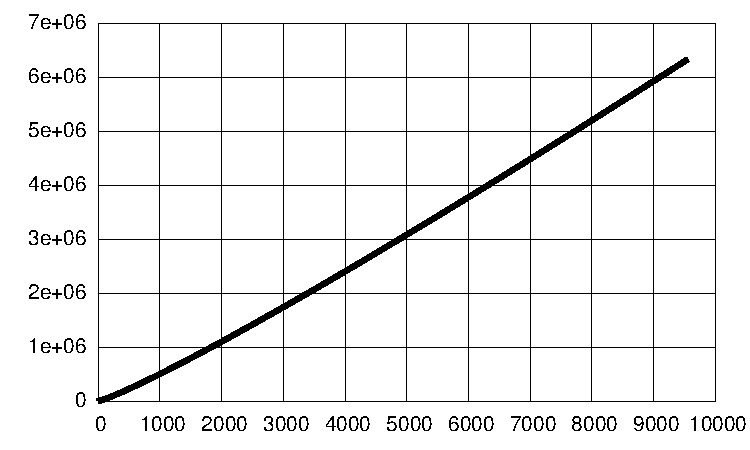
\includegraphics[width=0.44\columnwidth]{onln.pdf} &
    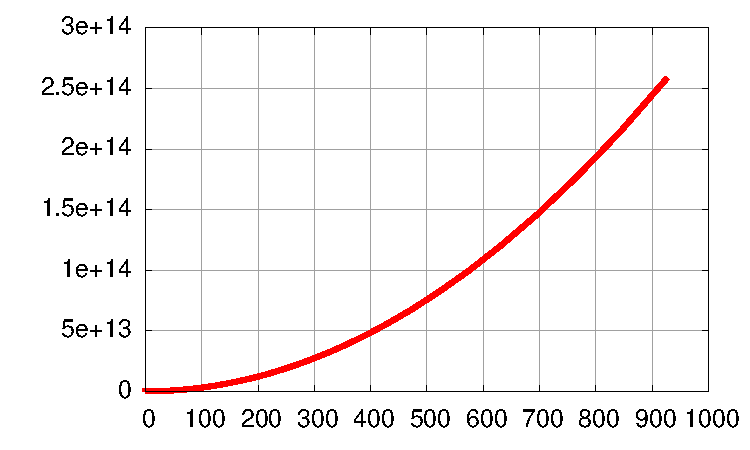
\includegraphics[width=0.44\columnwidth]{on2.pdf} \\
    \hline
    $O(N^2)$ &
    $T_X/N^2$ &
    $T_Y/N^2$ \\
    &
    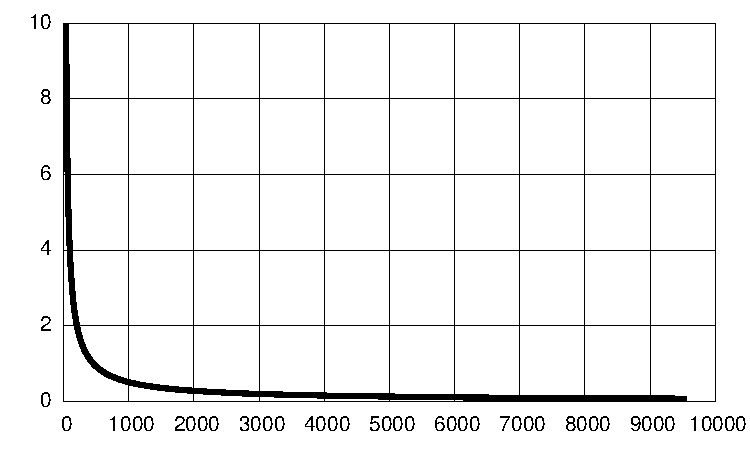
\includegraphics[width=0.44\columnwidth]{onln_n2.pdf} &
    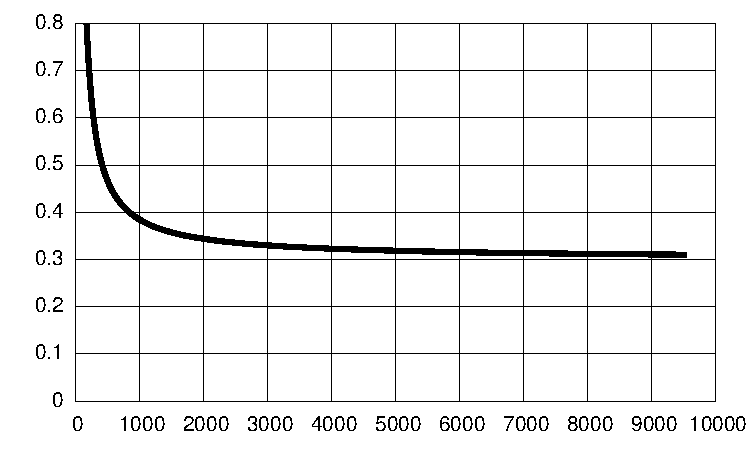
\includegraphics[width=0.44\columnwidth]{on2_n2.pdf} \\
    \hline
    $O(N\log N)$ &
    $T_X/(N\log N)$ &
    $T_Y/(N\log N)$ \\
    &
    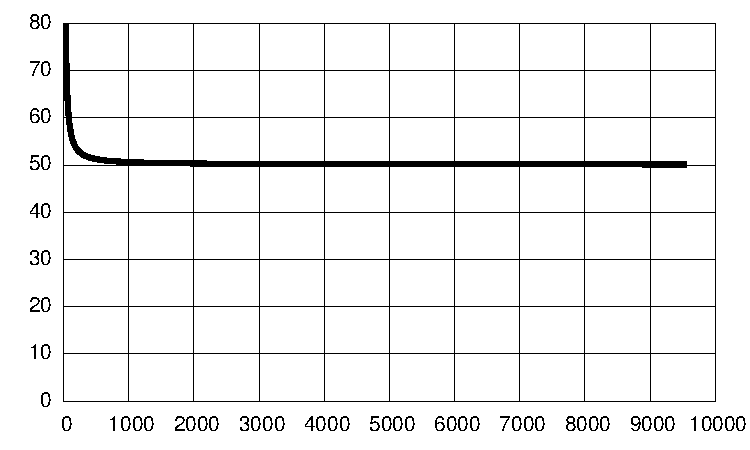
\includegraphics[width=0.44\columnwidth]{onln_nln.pdf} &
    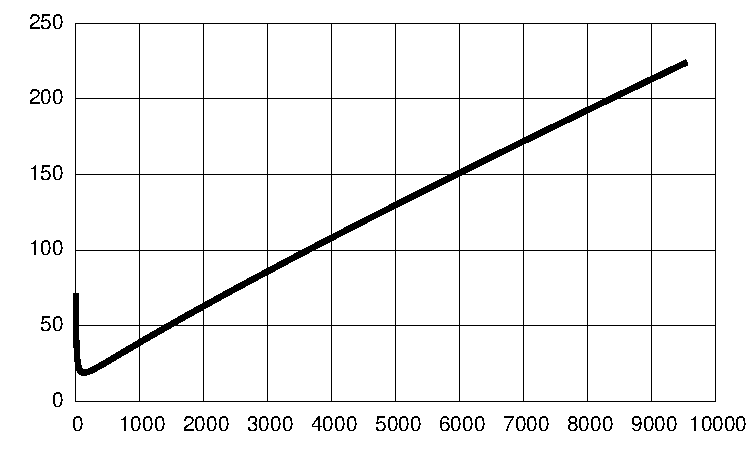
\includegraphics[width=0.44\columnwidth]{on2_nln.pdf} \\
    \hline
  \end{tabular}
\end{center}

\vfill

\noindent
Answer the following questions.

\begin{enumerate}
\item
  How big of a problem (approximately) can program \textbf{X} solve in $T=10^{14}$?
\item
  How big of a problem (approximately) can program \textbf{Y} solve in $T=10^{14}$?
\item
  What is the complexity class of program \textbf{X}?
\item
  What is the complexity class of program \textbf{Y}?
\item
  How long will program \textbf{X} run (approximately) for a problem of size $N=4000$?
\item
  How long will program \textbf{Y} run (approximately) for a problem of size $N=4000$?
\end{enumerate}

\end{document}
